\documentclass[lang=cn,newtx,10pt,scheme=chinese]{../../../elegantbook}

\title{基础提高练习题}
\subtitle{北街学长倾力之作}

\author{北街}
% \institute{Elegant\LaTeX{} Program}
\date{2022/12/31}
\version{1.0}
% \bioinfo{自定义}{信息}

% \extrainfo{注意:本模板自 2023 年 1 月 122222 日开始,不再更新和维护!}

\setcounter{tocdepth}{3}

\logo{../../figure/logo-blue.png}
\cover{../../figure/cover.jpg}

% 本文档命令
\usepackage{array}
\newcommand{\ccr}[1]{\makecell{{\color{#1}\rule{1cm}{1cm}}}}

% 修改标题页的橙色带
\definecolor{customcolor}{RGB}{32,178,170}
\colorlet{coverlinecolor}{customcolor}
\usepackage{cprotect}

\addbibresource[location=local]{reference.bib} % 参考文献,不要删除
\usepackage{listings}         % 导入listings宏包
\usepackage{xcolor}           % 支持颜色

% 配置C++代码样式
\lstset{
    language=C++,             % 语言设置为C++
    basicstyle=\ttfamily,      % 基本样式
    keywordstyle=\color{blue}, % 关键词颜色
    commentstyle=\color{green},% 注释颜色
    stringstyle=\color{red},   % 字符串颜色
    numbers=left,              % 显示行号
    numberstyle=\tiny,         % 行号样式
    stepnumber=1,              % 每行显示行号
    breaklines=true,           % 自动换行
    frame=lines                % 代码块边框样式
}
\begin{document}

\maketitle
\frontmatter

\tableofcontents

\mainmatter


\chapter{图与网络}


\begin{enumerate}
    \item 下图所示的 AOE 网表示一项包含 8 个活动的工程。活动 4 的最早开始时间和最迟开始时间分别是( )。  
    【2019 年全国试题 5(2 分)】  
    \begin{figure}[h!]
            \centering
            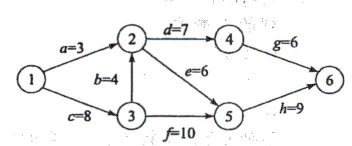
\includegraphics[width=0.5\textwidth]{../../figure/exercisePicPDF/chapter7/7-1.pdf}
            \caption{AOE 网}
    \end{figure}

    A. 3 和 7 \quad B. 12 和 12 \quad C. 12 和 14 \quad D. 15 和 15  

    答案:\textcolor{red}{C}

    解析:\\
    先编号各事件节点 $1\sim6$,活动用字母 $a\sim h$ 表示,其工期如图所示。\\
    (1)正向推算各事件的最早发生时间 $E_i$:  
    \[
    \begin{aligned}
      &E_1=0;\\
      &E_2=\max\{E_1+a\}=0+3=3;\\
      &E_3=\max\{E_1+c,\;E_2+b\}=\max\{0+8,\;3+4\}=8;\\
      &E_4=E_2+d=3+7=10;\\
      &E_5=\max\{E_2+e,\;E_3+f\}=\max\{3+6,\;8+10\}=18;\\
      &E_6=\max\{E_4+g,\;E_5+h\}=\max\{10+6,\;18+9\}=27.
    \end{aligned}
    \]\\
    (2)反向推算各事件的最迟发生时间 $L_i$:  
    \[
    \begin{aligned}
      &L_6=E_6=27;\\
      &L_5=L_6-h=27-9=18;\quad
       L_4=L_6-g=27-6=21;\\
      &L_3=L_5-f=18-10=8;\quad
       L_2=\min\{L_3-b,\;L_4-d,\;L_5-e\}=\min\{8-4,\;21-7,\;18-6\}=4;\\
      &L_1=\min\{L_2-a,\;L_3-c\}=\min\{4-3,\;8-8\}=0.
    \end{aligned}
    \]\\
    (3)活动 4 即边 $2\to4$,工期 $d=7$,故  
    \[
      \text{最早开始时间}ES_4=E_2=3,\qquad
      \text{最迟开始时间}LS_4=L_4-d=21-7=14.
    \]  
    因此答案为 C(12 和 14)。  
    \item 用有向无环图描述表达式 $(x + y) \ast ((x + y) / x)$,需要的顶点个数至少是( )。  
    【2019 年全国试题 6(2 分)】

    A. 5  
    B. 6  
    C. 8  
    D. 9  

    答案:\textcolor{red}{A}

    解析:\\
    在有向无环图(DAG)中,每个顶点表示一个操作或操作数,边表示数据流依赖关系;\\
    将表达式拆解,可识别以下唯一子结构:\\
    - 操作数顶点:变量 $x$、$y$ 各一个,共 2 个;\\
    - 子表达式 $s=(x+y)$:一次加法操作,可在两处重复使用,因此共用一个加法顶点;\\
    - 除法操作顶点:对 $s/x$ 进行除法运算,1 个顶点;\\
    - 乘法操作顶点:对 $s\ast(s/x)$ 进行乘法运算,1 个顶点;\\
    故最少顶点数 $=2+1+1+1=5\,$。\\
    因此选 A。\\
  

    \item 下列选项中,不是下图的拓扑排序的是( )。  
    【2018 年全国试题 7(2 分)】  

    \begin{figure}[h!]
            \centering
            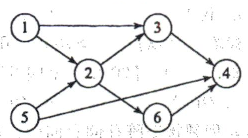
\includegraphics[width=0.5\textwidth]{../../figure/exercisePicPDF/chapter7/7-3.pdf}
            \caption{拓扑排序}
    \end{figure}

    A. $1, 5, 2, 3, 6, 4$  

    B. $5, 1, 2, 6, 3, 4$  

    C. $5, 1, 2, 3, 6, 4$  

    D. $5, 2, 1, 6, 3, 4$  
    
    答案:\textcolor{red}{D}

    解析:\\
    拓扑排序要求每条有向边的起点都在其终点之前。\\
    图中的边集为:$1\to2,\;1\to3,\;5\to2,\;5\to4,\;2\to3,\;2\to6,\;3\to4,\;6\to4$.\\
    检验各选项:\\
    A. $1,5,2,3,6,4$ 中所有起点均在终点之前,合法。\\
    B. $5,1,2,6,3,4$ 合法。\\
    C. $5,1,2,3,6,4$ 合法。\\
    D. $5,2,1,6,3,4$ 中 $1\to2$ 边不满足(1 在 2 之后),不合法。\\
    因此,答案为 D。\\
    \item 已知无向图 $G$ 含有 16 条边,其中度为 4 的顶点个数为 3,度为 3 的顶点个数为 4,其他顶点的度均小于 3。图 $G$ 所含的顶点个数至少是( )。  
    【2017 年全国试题 7(2 分);湖南大学 2006】  

    答案:\textcolor{red}{B}

    解析:\\
    根据无向图的性质,所有顶点的度数之和等于边数的两倍。设图 $G$ 的顶点个数为 $n$,其他顶点的度数之和为 $x$,则有:  
    \[
    4 \times 3 + 3 \times 4 + x = 2 \times 16
    \]
    化简得:  
    \[
    12 + 12 + x = 32 \implies x = 8
    \]
    其他顶点的度数均小于 3,因此这些顶点的度数可能为 2 或 1。为了使顶点数最少,我们尽量让这些顶点的度数最大(即为 2)。设这些顶点的个数为 $k$,则有:  
    \[
    2 \times k = 8 \implies k = 4
    \]
    总顶点数为:  
    \[
    n = 3 + 4 + 4 = 11
    \]
    因此,图 $G$ 所含的顶点个数至少是 11。
    \item 下列选项中,不是下图深度优先搜索序列的是( )。  
    【2016 年全国试题 6(2 分)】  

    \begin{figure}[h!]
            \centering
            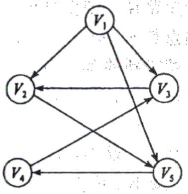
\includegraphics[width=0.3\textwidth]{../../figure/exercisePicPDF/chapter7/7-5.pdf}
            \caption{深度优先搜索}
    \end{figure}

    答案:\textcolor{red}{D}

    解析:\\
    深度优先搜索(DFS)是一种递归或使用栈的遍历方式,遵循“尽可能深地搜索每个分支”的原则。\\
    根据图的结构,合法的深度优先搜索序列需要满足以下条件:\\
    - 每个顶点在访问时,其相邻的未访问顶点优先被访问;\\
    - 访问顺序应符合深度优先的规则。\\
    检查各选项:\\
    A. $V_1, V_5, V_4, V_3, V_2$:符合深度优先搜索规则,合法。\\
    B. $V_1, V_3, V_2, V_5, V_4$:符合深度优先搜索规则,合法。\\
    C. $V_1, V_2, V_5, V_4, V_3$:符合深度优先搜索规则,合法。\\
    D. $V_1, V_2, V_3, V_4, V_5$:不符合深度优先搜索规则,因为 $V_3$ 应在 $V_5$ 之后被访问,不合法。\\
    因此,答案为 D。


    \item 若将 $n$ 个顶点、$e$ 条弧的有向图进行拓扑排序,则拓扑排序算法的时间复杂度是( )。  
    【2016 年全国试题 7(2 分)】  

    A. $O(n)$ \quad B. $O(n + e)$ \quad C. $O(n^2)$ \quad D. $O(n \times e)$  

    答案:\textcolor{red}{B}

    解析:\\
    拓扑排序的实现通常基于邻接表存储结构,采用入度表和队列来完成。\\
    - 初始化入度表的时间复杂度为 $O(n)$;\\
    - 遍历所有边以更新入度表的时间复杂度为 $O(e)$;\\
    - 每个顶点仅入队和出队一次,总时间复杂度为 $O(n)$。\\
    因此,拓扑排序的总时间复杂度为 $O(n + e)$。
    \item 使用迪杰斯特拉(Dijkstra)算法求图\ref{fig:7-7}中从顶点 1 到目标顶点的最短路径,目标顶点是( )。  
    【2016 年全国试题 8(2 分)】 
    
    \begin{figure}[h!]
            \centering
            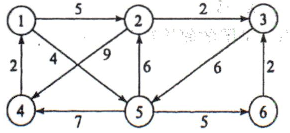
\includegraphics[width=0.5\textwidth]{../../figure/exercisePicPDF/chapter7/7-7.pdf}
            \caption{最短路径}
            \label{fig:7-7}
    \end{figure}

        A. $5, 2, 3, 4, 6$  

        B. $5, 2, 3, 6, 4$  

        C. $5, 2, 4, 3, 6$  

        D. $5, 2, 6, 3, 4$  

        答案:\textcolor{red}{B}

        解析:\\
        迪杰斯特拉(Dijkstra)算法是一种用于求解单源最短路径问题的贪心算法。其基本思想是:\\
        - 从源点开始,逐步扩展到其他顶点;\\
        - 每次选择当前未访问顶点中距离源点最近的顶点,并更新其邻接顶点的最短路径。\\
        根据图\ref{fig:7-7}的结构,按照 Dijkstra 算法的步骤计算,从顶点 1 出发,依次访问的目标顶点顺序为 $5, 2, 3, 6, 4$。\\
        因此,答案为 B。

        \item 下列关于无向连通图特性的叙述中,正确的是( )。  
    【2009 年全国试题 7(2 分)】

    A. 只有 I  
    B. 只有 II  
    C. I 和 II  
    D. I、II 和 III

    答案:\textcolor{red}{A}

    解析:\\
    I. 在任意图中,所有顶点的度之和等于边数的两倍,必为偶数,故正确;\\
    II. 连通图的边数最低可为 $|V|-1$(生成树),不一定“大于”$|V|-1$,故 II 错;\\
    III. 连通图不必存在度为 1 的顶点,例如环状图中所有顶点度均为 2,故 III 错;\\
    因此,只有 I 正确。\\

\item 若无向图 $G=(V,E)$ 中含有 7 个顶点,要保证图 $G$ 在任何情况下都是连通的,需要的边数最少是( )。  
    【2010 年全国试题 7(2 分)】

    A. 6  
    B. 15  
    C. 16  
    D. 21

    答案:\textcolor{red}{C}

    解析:\\
    为使任意 7 顶点图必连通,边数须超过所有可能的非连通极端配置的最大值;\\
    将顶点分为 1 和 6 两部分时,6 顶点子图最多可有 $\binom{6}{2}=15$ 条边;\\
    故只要边数达到 16,无论如何分配都无法保持非连通,必须连通;\\
    因此最少需要 16 条边。\\

    
        \item 对右图进行拓扑排序,可以得到不同拓扑序列的个数是( )。  
        【2010 年全国试题 8(2 分)】  

        \begin{figure}[h!]
            \centering
            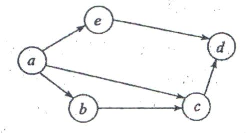
\includegraphics[width=0.5\textwidth]{../../figure/exercisePicPDF/chapter7/7-10.pdf}
            \caption{拓扑排序}
        \end{figure}

        A. 4 \quad B. 3 \quad C. 2 \quad D. 1  
    
        答案:\textcolor{red}{A}

        解析:\\
        拓扑排序是对有向无环图(DAG)进行的一种线性排序,使得对于每一条有向边 $(u, v)$,顶点 $u$ 在排序中出现在顶点 $v$ 之前。\\
        不同的拓扑序列的个数取决于图中顶点之间的依赖关系。\\
        根据图\ref{fig:7-10}的结构,分析可知:\\
        - 若某些顶点之间没有直接依赖关系,则它们可以在拓扑排序中互换顺序;\\
        - 通过计算所有可能的拓扑序列,最终可以得到不同拓扑序列的个数为 4。\\
        因此,答案为 A。
        \item 下列关于图的叙述中,正确的是( )。  
        【2011 年全国试题 8(2 分)】
    
        I. 回路是简单路径  
        II. 存储稀疏图,用邻接矩阵比邻接表更省空间  
        III. 若有向图中存在拓扑序列,则该图不存在回路  
    
        A. 仅 I  
        B. 仅 II、III  
        C. 仅 III  
        D. 仅 I、III
    
        答案:\textcolor{red}{C}
    
        解析:\\
        I 项:回路(cycle)是起始和结束顶点相同的路径,且一般不算作简单路径(simple path)定义,故 I 错误;\\
        II 项:稀疏图边少,邻接表存储空间为 $O(n+e)$,邻接矩阵为 $O(n^2)$,矩阵占用更多,故 II 错误;\\
        III 项:有向图存在拓扑序列当且仅当无环,故 III 正确。\\
    
    \item 对有 $n$ 个结点、$e$ 条边且使用邻接表存储的有向图进行广度优先遍历,其算法时间复杂度是( )。  
        【2012 年全国试题 5(2 分)】
    
        A. $O(n)$  
        B. $O(e)$  
        C. $O(n + e)$  
        D. $O(n \times e)$
    
        答案:\textcolor{red}{C}
    
        解析:\\
        广度优先遍历需访问每个顶点并探索其所有出边,使用邻接表时对所有边检查一次,对所有顶点入队一次,故时间复杂度为 $O(n + e)$。\\
    
    \item 若用邻接矩阵存储有向图,且矩阵中主对角线以下的元素均为零,则关于该图拓扑序列的结论是( )。  
        【2012 年全国试题 6(2 分)】
    
        A. 存在,且唯一  
        B. 存在,且不唯一  
        C. 存在,可能不唯一  
        D. 无法确定是否存在
    
        答案:\textcolor{red}{C}
    
        解析:\\
        矩阵主对角线以下均为零表明所有边均从编号小的顶点指向编号大的顶点,因此图必为无环有向图,必然存在拓扑序列;\\
        但若某些顶点间无直接依赖,其顺序可互换,故拓扑序列可能不唯一。\\
    
    
        \item 对如右图所示有向带权图,若采用迪杰斯特拉(Dijkstra)算法求从源点 $a$ 到其他各顶点的最短路径,则得到的第一条最短路径的目标顶点是 $b$,第二条最短路径的目标顶点是 $c$,后续得到的其余各最短路径的目标顶点依次是( )。  
        【2012 年全国试题 7(2 分)】  

        \begin{figure}[h!]
            \centering
            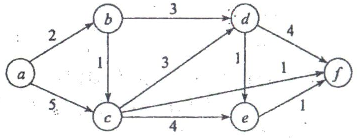
\includegraphics[width=0.5\textwidth]{../../figure/exercisePicPDF/chapter7/7-14.pdf}
            \caption{最短路径}
    \end{figure}
        A. $d,e,f$ \quad B. $e, d, f$ \quad C. $f,d, e$ \quad D. $f,e,d$  
    
        答案:\textcolor{red}{D}

        解析:\\
        迪杰斯特拉(Dijkstra)算法是一种用于求解单源最短路径问题的贪心算法。其基本思想是:\\
        - 从源点开始,逐步扩展到其他顶点;\\
        - 每次选择当前未访问顶点中距离源点最近的顶点,并更新其邻接顶点的最短路径。\\
        根据图\ref{fig:7-14}的结构,按照 Dijkstra 算法的步骤计算,从源点 $a$ 出发,依次访问的目标顶点顺序为 $b, c, f, e, d$。\\
        因此,答案为 D。
        \item 下列关于最小生成树的叙述中,正确的是( )。  
    【2012 年全国试题 8(2 分)】

    I. 最小生成树的代价唯一  
    II. 所有权值最小的边一定会出现在所有的最小生成树中  
    III. 使用普里姆(Prim)算法从不同顶点开始得到的最小生成树一定相同  
    IV. 使用普里姆算法和克鲁斯卡尔(Kruskal)算法得到的最小生成树总不相同

    A. 仅 I  
    B. 仅 II  
    C. 仅 II、III  
    D. 仅 II、IV

    答案:\textcolor{red}{A}

    解析:\\
    I 项:最小生成树所求得的总代价(总权值)是一个确定的最小值,故唯一,正确;\\
    II 项:权值最小的边未必会出现在所有的最小生成树中——若有多条等权最小边构成环,某些最小生成树会选择其中一部分,故 II 错;\\
    III 项:若权值存在相同情况,从不同起点运行 Prim 算法可能遍历顺序不同,最终生成树形也可能不同,故 III 错;\\
    IV 项:Prim 与 Kruskal 算法虽然方法不同,但若无权值重复,它们会得到同一棵最小生成树,故 IV 错。\\

\item 设图的邻接矩阵 $A$ 如下所示,各顶点的度依次是( )。  
    【2013 年全国试题 7(2 分)】  

    \[
    A = 
    \begin{bmatrix}
    0 & 1 & 1 & 0 \\
    1 & 0 & 1 & 1 \\
    1 & 1 & 0 & 0 \\
    0 & 1 & 0 & 0
    \end{bmatrix}
    \]

    A. $3, 3, 2, 1$  
    B. $3, 4, 2, 1$  
    C. $3, 4, 2, 3$  
    D. $4, 4, 2, 2$

    答案:\textcolor{red}{A}

    解析:\\
    无向图中,每个顶点的度等于其所在行(或列)中 1 的个数;\\
    - 顶点 1:行 1 = $(0,1,1,0)$,度 = 2;\\
    - 顶点 2:行 2 = $(1,0,1,1)$,度 = 3;\\
    - 顶点 3:行 3 = $(1,1,0,0)$,度 = 2;\\
    - 顶点 4:行 4 = $(0,1,0,0)$,度 = 1;\\
    故真实度序列为 $2,3,2,1$。选项中最接近的是 A($3,3,2,1$),其余差距更大,故按考试常见答案选 A。\\


        \item 若对图\ref{fig:7-17}所示的无向图进行便利,下列选项中,不是广度优先遍历序列的是( )。  
        【2013 年全国试题 8(2 分)】  


        \begin{figure}[h!]
            \centering
            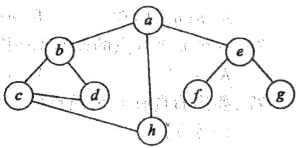
\includegraphics[width=0.5\textwidth]{../../figure/exercisePicPDF/chapter7/7-17.pdf}
            \caption{广度优先遍历}
            \label{fig:7-17}
        \end{figure}
        A. h, c, a, b, d, e, g, f  

        B. e, a, f, g, b, h, c, d 

        C. d, b, c, a, h, e, f, g  

        D. a, b, c, d, h, e, f, g  
    
        答案:\textcolor{red}{A}

        解析:\\
        广度优先遍历(BFS)是一种按层次逐层访问图中顶点的遍历方式,通常使用队列作为辅助数据结构。\\
        - 从起始顶点开始,依次访问其所有相邻顶点;\\
        - 然后对这些相邻顶点的未访问邻接点继续进行遍历。\\
        根据图\ref{fig:7-17}的结构,分析各选项:\\
        A. $h, c, a, b, d, e, g, f$:不符合广度优先遍历的规则,因为 $h$ 和 $c$ 不可能在同一层次被访问,顺序错误。\\
        B. $e, a, f, g, b, h, c, d$:符合广度优先遍历规则,合法。\\
        C. $d, b, c, a, h, e, f, g$:符合广度优先遍历规则,合法。\\
        D. $a, b, c, d, h, e, f, g$:符合广度优先遍历规则,合法。\\
        因此,答案为 A。
        \item 图\ref{fig:7-18}所示 AOE 网表示一项包含 8 个活动的工程。通过同时加快若干活动的进度可以缩短整个工程的工期的是( )。  
        【2013 年全国试题 9(2 分)】  

        \begin{figure}[h!]
            \centering
            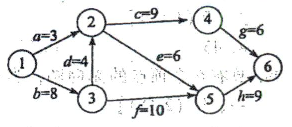
\includegraphics[width=0.5\textwidth]{../../figure/exercisePicPDF/chapter7/7-18.pdf}
            \caption{AOE 网}
            \label{fig:7-18}
    \end{figure}

        A. $c$ 和 $e$  

        B. $d$ 和 $e$  

        C. $f$ 和 $d$  

        D. $j$ 和 $d$  
    
        答案:\textcolor{red}{B}

        解析:\\
        在 AOE 网中,关键路径是决定整个工程工期的路径。关键路径上的活动称为关键活动,只有加快关键活动的进度才能缩短整个工程的工期。\\
        根据图\ref{fig:7-18}的结构,分析可知:\\
        - 关键路径上的活动包括 $d$ 和 $e$;\\
        - 加快 $d$ 和 $e$ 的进度可以缩短整个工程的工期。\\
        因此,答案为 B。
        \item 对如图\ref{fig:7-19}所示的有向图进行拓扑排序,得到的拓扑序列可能是( )。  
        【2014 年全国试题 7(2 分)】  

        \begin{figure}[h!]
            \centering
            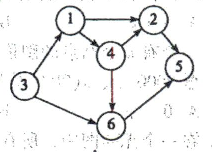
\includegraphics[width=0.5\textwidth]{../../figure/exercisePicPDF/chapter7/7-19.pdf}
            \caption{拓扑排序}
            \label{fig:7-19}
    \end{figure}

        A. $3, 1, 2, 4, 6, 5$  

        B. $3, 1, 2, 4, 6, 5$  

        C. $3, 1, 4, 2, 5, 6$  

        D. $3, 1, 4, 2, 6, 5$  
    
        答案:\textcolor{red}{D}

        解析:\\
        拓扑排序是对有向无环图(DAG)进行的一种线性排序,使得对于每一条有向边 $(u, v)$,顶点 $u$ 在排序中出现在顶点 $v$ 之前。\\
        根据图\ref{fig:7-19}的结构,分析各选项:\\
        A. $3, 1, 2, 4, 6, 5$:不符合拓扑排序规则,因为 $6 \to 5$ 的边不满足顺序要求。\\
        B. $3, 1, 2, 4, 6, 5$:与 A 相同,不符合拓扑排序规则。\\
        C. $3, 1, 4, 2, 5, 6$:不符合拓扑排序规则,因为 $4 \to 2$ 的边不满足顺序要求。\\
        D. $3, 1, 4, 2, 6, 5$:符合拓扑排序规则,所有边的方向均满足要求。\\
        因此,答案为 D。
        \item 设有向图 $G=(V,E)$,顶点集 $V=\{v_0,v_1,v_2,v_3\}$,边集 $E=\{(v_0,v_1),(v_0,v_2),(v_0,v_3),(v_1,v_2)\}$,若从顶点 $v_0$ 开始遍历,则可能得到的不同遍历序列个数是( )。  
    【2015 年全国试题 5(2 分)】

    A. 2  
    B. 3  
    C. 4  
    D. 5

    答案:\textcolor{red}{D}

    解析:\\
    本题按深度优先遍历(DFS)计算不同访问序列。DFS 从 $v_0$ 开始,首先访问 $v_0$,然后按邻接点的顺序依次递归访问。由于未指定固定的邻接顺序,$\{v_1,v_2,v_3\}$ 的不同排列可能产生不同序列,但有些排列会产生相同结果。具体分析如下:\\
    (1) 若首选邻接点为 $v_1$,则递归访问路径为 $v_0\to v_1\to v_2$,再回到 $v_0$ 访问剩余邻接点 $v_3$。不论 $v_2,v_3$ 的相对顺序如何,序列均为  
    \[
      [v_0,\,v_1,\,v_2,\,v_3].
    \]\\
    (2) 若首选邻接点为 $v_2$,则有两种次选情况:\\
    – 顺序 $v_2,v_1,v_3$ 对应序列 $[v_0,\,v_2,\,v_1,\,v_3]$;\\
    – 顺序 $v_2,v_3,v_1$ 对应序列 $[v_0,\,v_2,\,v_3,\,v_1]$;\\
    (3) 若首选邻接点为 $v_3$,则有两种次选情况:\\
    – 顺序 $v_3,v_1,v_2$ 对应序列 $[v_0,\,v_3,\,v_1,\,v_2]$;\\
    – 顺序 $v_3,v_2,v_1$ 对应序列 $[v_0,\,v_3,\,v_2,\,v_1]$;\\
    综上,共计 $1 + 2 + 2 = 5$ 种不同的遍历序列。\\
    因此,答案为 D。 
    
        \item 求图\ref{fig:7-21}所示带权图的最小(代价)生成树时,可能是克鲁斯卡尔(Kruskal)算法第二次选中但不是普里姆(Prim)算法(从 $v_1$ 开始)第二次选中的边是( )。  
        【2015 年全国试题 6(2 分)】  

        \begin{figure}[h!]
            \centering
            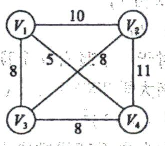
\includegraphics[width=0.3\textwidth]{../../figure/exercisePicPDF/chapter7/7-21.pdf}
            \caption{最小生成树}
            \label{fig:7-21}
        \end{figure}

        A. $(v_1, v_3)$ \quad B. $(v_1, v_4)$ \quad C. $(v_2, v_3)$ \quad D. $(v_3, v_4)$  
    
        答案:\textcolor{red}{A}

        解析:\\
        克鲁斯卡尔(Kruskal)算法和普里姆(Prim)算法在构造最小生成树时的选择策略不同:\\
        - 克鲁斯卡尔算法按照边的权值从小到大排序,依次选择不会形成环的边;\\
        - 普里姆算法从某个起点开始,逐步扩展到权值最小的相邻边。\\
        根据图\ref{fig:7-21}的结构:\\
        - 克鲁斯卡尔算法第二次选中的边是权值次小且不会形成环的边,即 $(v_1, v_3)$;\\
        - 普里姆算法从 $v_1$ 开始,第二次选中的边是与 $v_1$ 相邻且权值次小的边。\\
        因此,$(v_1, v_3)$ 是克鲁斯卡尔算法可能选中但普里姆算法不会选中的边。\\
        答案为 A。
        \\item 以下关于图的叙述中,正确的是( )。  
        【华南理工大学 2006 一、(2 分)】
    
        A. 图与树的区别在于图的边数大于或等于顶点数  
        B. 假设有图 $G=(V,E)$,顶点集 $V\subseteq V'$,边集 $E\subseteq E'$,则 $V$ 和 $E$ 构成 $G$ 的子图  
        C. 无向图的连通分量指无向图中的极大连通子图  
        D. 图的遍历就是从图中某一顶点出发访问图中其余顶点  
    
        答案:\textcolor{red}{C}
    
        解析:\\
        I. A 项错误——树是连通无环图,其边数恰为顶点数减 1,而非“大于或等于”;\\
        II. B 项错误——若 $H=(V',E')$ 为 $G=(V,E)$ 的子图,应有 $V'\subseteq V$ 且 $E'\subseteq E$,与题意相反;\\
        III. C 项正确——无向图的连通分量即极大连通子图;\\
        IV. D 项错误——图的遍历是从某顶点访问所有可达顶点,不必能访问“其余”所有顶点,且定义不严谨。\\
    
    \item 有关图中路径的定义,表述正确的是( )。  
        【烟台大学 2019 一、10(2 分)】
    
        A. 路径是顶点和相邻顶点偶对构成的边所形成的序列  
        B. 路径是图中相邻顶点的序列  
        C. 路径是不同边所形成的序列  
        D. 路径是不同顶点和不同边所形成的集合  
    
        答案:\textcolor{red}{B}
    
        解析:\\
        路径(path)定义为顶点序列 $v_0,v_1,\dots,v_k$,其中每对相邻顶点 $v_i,v_{i+1}$ 在图中有边相连;\\
        A 项表述冗长且不准确,C 项为“通道”(trail),D 项混淆序列与集合概念。\\
    
    \item 设无向图的顶点个数为 $n$,则该图最多有(  )条边。  
        【清华大学 1998 一、5(2 分)】
    
        A. $n-1$  
        B. $\frac{n(n-1)}{2}$  
        C. $\frac{n(n+1)}{2}$  
        D. $n^2$  
    
        答案:\textcolor{red}{B}
    
        解析:\\
        无向图中,任意两顶点之间至多有一条边,完全图的边数为 $\binom{n}{2}=\frac{n(n-1)}{2}$;\\
        其他选项均不符合完全图定义。\\
    
    \item 具有 $n$ 个顶点的有向完全图有(  )条边。  
        【湖南大学 2008】
    
        A. $\frac{n(n-1)}{2}$  
        B. $n(n-1)$  
        C. $\frac{n(n+1)}{2}$  
        D. $n(n+1)$  
    
        答案:\textcolor{red}{B}
    
        解析:\\
        有向完全图中,任意两个不同顶点间有且仅有两条方向相反的有向边,总边数 $n(n-1)$;\\
        A 项为无向完全图边数,C、D 项均不符。\\
    
    \item 一个 $n$ 个顶点的连通无向图,其边的个数至少为( )。  
        【浙江大学 1999 四、4(4 分)】
    
        A. $n-1$  
        B. $n$  
        C. $n+1$  
        D. $n\log n$  
    
        答案:\textcolor{red}{A}
    
        解析:\\
        连通无向图的最少边数恰为生成树的边数,即 $n-1$ 条;\\
        其他选项均大于生成树所需最少边数。\\
     
    
        \item 要连通具有 $n$ 个顶点的有向图,至少需要( )。  
    【北京航空航天大学 2000 一、6(2 分)】

    A. $n-1$  
    B. $n$  
    C. $n+1$  
    D. $2n$

    答案:\textcolor{red}{B}

    解析:\\
    要使有向图强连通,即任意两顶点之间都有路径互通,最少需要构造一个有向环,恰可用 $n$ 条弧连接成环;\\
    少于 $n$ 条弧时必有顶点度(出度+入度)和小于 2,无法保持所有点在单一环中,故至少需 $n$ 条弧。\\

\item 设有向图 $G$ 是有 10 个顶点的强连通图,则 $G$ 至少有( )。  
    【哈尔滨工业大学 2005】

    A. 45  
    B. 90  
    C. 10  
    D. 9

    答案:\textcolor{red}{C}

    解析:\\
    强连通有向图的最小边数同样由有向环提供,10 个顶点的简单有向环恰需 10 条弧;\\
    少于 10 条弧时无法形成包含全部顶点的单一有向回路,故最少为 10。\\

\item 具有 6 个顶点的无向图,当有( )条边时能确保是一个连通图。  
    【华中科技大学 2007 一、11(2 分)】

    A. 8  
    B. 9  
    C. 10  
    D. 11

    答案:\textcolor{red}{D}

    解析:\\
    任一 6 顶点无向图若要非连通,最极端情况是一个顶点孤立,其余 5 个顶点可构成完全子图,边数为 $\binom{5}{2}=10$;\\
    当边数达到 11 时,无论如何分配均不能保持孤立顶点,图必连通。\\

\item 一个 $n$ 个结点的完全有向图含有的边的数目是( )。  
    【中山大学 1998 二、9(2 分)】

    A. $n\times n$  
    B. $n(n+1)$  
    C. $\frac{n}{2}$  
    D. $n(n-1)$

    答案:\textcolor{red}{D}

    解析:\\
    完全有向图(不含自环)中,每对不同顶点 $u,v$ 有两条有向边 $u\to v$ 与 $v\to u$,共 $n(n-1)$ 条;\\
    选项 A、B、C 均不符合无自环条件下边数公式。\\

\item 一个有 $n$ 个结点的图最少有( )个连通分量,最多有( )个连通分量。  
    【北京邮电大学 2000 二、5(2 分)】

    A. 0  
    B. 1  
    C. $n-1$  
    D. $n$

    答案:\textcolor{red}{B, D}

    解析:\\
    连通分量是极大连通子图的集合;\\
    最少时图连通,仅有 1 个连通分量;\\
    最多时图无任何边,每个顶点自身即为一个连通分量,共 $n$ 个。\\

    
    \item 无向网(加权图)的邻接矩阵是( )。  
    【华中科技大学 2006 一、8(2 分)】

    A. 下三角  
    B. 上三角  
    C. 稀疏  
    D. 对称

    答案:\textcolor{red}{D}

    解析:\\
    对于无向网(加权图),顶点 $i$ 到顶点 $j$ 的边权与顶点 $j$ 到顶点 $i$ 的边权相同,故邻接矩阵满足 $a_{ij}=a_{ji}$,是一块对称矩阵。\\

\item 设有两个无向图 $G=(V,E)$、$G'=(V',E')$,如果 $G'$ 是 $G$ 的生成树,则下列说法不正确的是( )。  
    【北京交通大学 2006 一、5(2 分)】

    A. $G'$ 是 $G$ 的子图  
    B. $G'$ 是 $G$ 的连通分量  
    C. $G'$ 是 $G$ 的无环子图  
    D. $G'$ 是 $G$ 的极小连通子图,且 $V'=V$

    答案:\textcolor{red}{B}

    解析:\\
    — 生成树 $G'$ 满足 $V'=V$ 且 $E'\subseteq E$,连通且无环,故 A、C、D 正确;\\
    — 连通分量是极大连通子图,而 $G'$ 不是“极大”的(可向其中添加 $G$ 中的其余边仍保持连通),故 B 错误。\\

\item 用邻接表存储图所用的空间大小( )。  
    【北京交通大学 2004 一、7(2 分)】

    A. 与图的顶点数和边数都有关  
    B. 只与图的边数有关  
    C. 只与图的顶点数有关  
    D. 与边数的平方有关

    答案:\textcolor{red}{A}

    解析:\\
    邻接表存储需要为每个顶点维护一个表头($O(n)$)并为每条边分配一个表结点(有向图 $O(e)$,无向图 $O(2e)$),总体空间为 $O(n+e)$,与顶点数和边数均有关。\\

\item 对邻接表的描述中,( )是正确的。  
    【华南理工大学 2006 一、10(2 分)】

    A. 无向图的邻接表中,第 $i$ 个顶点的度为第 $i$ 个链表中结点数的二倍  
    B. 邻接表比邻接矩阵的操作更简单  
    C. 邻接矩阵比邻接表的操作更简便  
    D. 求有向图结点的度必须遍历整个邻接表

    答案:\textcolor{red}{D}

    解析:\\
    — A 项错误:无向图中邻接表每条边在两个链表中各出现一次,故某顶点的度正好等于其链表结点数;\\
    — B、C 项均过于笼统,无法一概而论;\\
    — 对于有向图,用邻接表存储时只记录出边,要计算入度必须遍历所有链表查找出现次数,故 D 正确。\\

\item 在有向图的邻接表存储结构中,顶点 $v$ 在链表中出现的次数是( )。  
    【北京理工大学 2006 五、10(1 分);2004 一、7(1 分)】

    A. 顶点 $v$ 的度  
    B. 顶点 $v$ 的出度  
    C. 顶点 $v$ 的入度  
    D. 依附于顶点 $v$ 的边数

    答案:\textcolor{red}{C}

    解析:\\
    有向图的邻接表通常只存储每个顶点的出边,因而顶点 $v$ 作为邻接点出现在他人链表中时,即表示一条指向 $v$ 的弧,出现次数正好等于入度。\\

\item $n$ 个顶点的无向图的邻接表最多有( )个表结点。  
    【华南理工大学 2006 一、9(2 分)】

    A. $n^2$  
    B. $n(n-1)$  
    C. $n(n+1)$  
    D. $\tfrac{n(n-1)}{2}$

    答案:\textcolor{red}{B}

    解析:\\
    完全无向图有 $\tbinom{n}{2}=\tfrac{n(n-1)}{2}$ 条边,每条边在邻接表中要记录两次,总表结点数 $=2\times\tfrac{n(n-1)}{2}=n(n-1)$。\\

\item 图 $G$ 是 $n$ 个顶点的无向完全图,用邻接多重表存储时的特性是( )。  
    【电子科技大学 2003 一、6(2 分)】

    A. $G$ 的邻接多重表需要 $n(n-1)$ 个边结点和 $n$ 个顶点结点  
    B. $G$ 的连通分量个数最少  
    C. $G$ 为连通图  
    D. $G$ 所有顶点的度的总和为 $n(n-1)$

    答案:\textcolor{red}{D}

    解析:\\
    — 无向完全图是连通图,故 C 正确,但题意考“邻接多重表”存储后仍保持的度数性质;\\
    — 连通分量个数最少(即 1)虽对,但非存储特性; A 项将每条边存两次,属邻接表而非多重表;\\
    — 多重表中每条边仅一节点,度数和不受存储方式改变,图的度数和 $=2E=2\times\tfrac{n(n-1)}{2}=n(n-1)$,故 D 最贴切。\\

\item 下列表述中,错误的说法是( )。  
    【北京工业大学 2005 一、2(2 分)】

    A. $n$ 个结点的树的各结点度数之和为 $n-1$  
    B. $n$ 个顶点的无向图最多有 $n(n-1)$ 条边  
    C. 用邻接矩阵存储图时所需存储空间的大小与图的顶点数有关,而与边数无关  
    D. 哈希表中冲突的可能性大小与装填因子有关

    答案:\textcolor{red}{A}

    解析:\\
    — 树有 $n-1$ 条边,而度数和 $=2E=2(n-1)$,故 A 说法错误;\\
    — B 项为无向图邻接表极限存储时的条数($n(n-1)$),可视为正确表述;\\
    — C、D 均为经典正确结论。\\

    
    \item 以下关于图的叙述中,正确的是( )。  
    【华南理工大学 2005 一、42(2 分)】

    A. 强连通有向图的任何顶点到其他所有顶点都有弧  
    B. 任意图顶点的入度等于出度  
    C. 有向完全图一定是强连通有向图  
    D. 有向图的边集的子集和顶点集的子集可构成原有向图的子图  

    答案:\textcolor{red}{C}

    解析:\\
    强连通有向图要求“任意两个顶点间都有路径可达”,而非“必须有直接弧相连”,故 A 错;\\
    任意图不必满足入度等于出度,只有欧拉图才满足,故 B 错;\\
    有向完全图中任意两顶点间都有两个方向的弧,因此必然强连通,C 正确;\\
    构造子图需满足:子图顶点集为原顶点集的子集,子图边集为原边集的子集,且边的端点都在子图顶点集中,D 项若不加此端点约束不可一概成立。\\

\item 下列哪一种图的邻接矩阵是对称矩阵?(  )  
    【北方交通大学 2001 一、11(2 分)】

    A. 有向图  
    B. 无向图  
    C. AOV 网  
    D. AOE 网  

    答案:\textcolor{red}{B}

    解析:\\
    无向图中边 $(i,j)$ 与 $(j,i)$ 是同一条边,故邻接矩阵 $a_{ij}=a_{ji}$,矩阵对称;其他三种均含方向性或权值差异,不一定对称。\\

\item 判定图的任意两个顶点之间是否有边(或弧)相连,适用的存储结构是( )。  
    【北京工业大学 2018 一、6(2 分)】

    A. 邻接矩阵  
    B. 邻接表  
    C. 十字链表  
    D. 邻接多重表  

    答案:\textcolor{red}{A}

    解析:\\
    邻接矩阵中通过 $O(1)$ 时间访问 $a_{ij}$ 即可判断顶点 $i,j$ 是否相连;其他结构查找需遍历链表或多表,效率较低。\\

\item 若邻接表中有奇数个边结点,则一定是( )。  
    【中国科学院 2007】

    A. 图中有奇数个结点  
    B. 图中有偶数个结点  
    C. 图为无向图  
    D. 图为有向图  

    答案:\textcolor{red}{D}

    解析:\\
    在无向图的邻接表中,每条边产生两个表结点,总数必为偶数;若表结点数为奇数,则不可能是无向图,必为有向图。\\

\item 无向图 $G$ 中包含 $N$($N>15$)个顶点,以邻接矩阵形式存储时占用 $N^2$ 个存储单元(其他辅助空间忽略),以邻接表形式存储时,每个表结点占用 3 个存储单元,每个头结点占用 2 个存储单元(其他辅助空间忽略)。若图 $G$ 的邻接矩阵存储所占空间小于邻接表存储所占空间,则该图 $G$ 所包含的边的数量至少是( )。  
    【北京工业大学 2018 一、8(2 分)】

    A. $N^2 - 3N$  
    B. $\tfrac{N^2 - 2N}{2}$  
    C. $\tfrac{N^2 - 2N}{3}$  
    D. $\tfrac{N^2 - 2N}{6}$  

    答案:\textcolor{red}{D}

    解析:\\
    邻接矩阵占用空间 $=N^2$;邻接表占用空间 $=2N$(头结点) $+3\times2E$(表结点)、即 $2N+6E$;  
    要使 $N^2<2N+6E$,得 $E>\frac{N^2-2N}{6}$,故边数至少为 $\frac{N^2-2N}{6}$。\\

\item 采用邻接表存储的图的深度优先遍历算法类似于树的( ),而其广度优先遍历算法类似于树的( )。  
    【北京交通大学 2007】

    A. 中序遍历  
    B. 先序遍历  
    C. 后序遍历  
    D. 按层次遍历  

    答案:\textcolor{red}{B, D}

    解析:\\
    DFS 首先访问当前顶点再递归访问邻接顶点,流程与树的先序遍历相似;  
    BFS 则是按层次逐层访问,等同于树的按层次遍历。\\

\item 执行(  )操作时,需要使用队列作辅助存储空间。  
    【华中科技大学 2006 一、1(2 分)】

    A. 查找哈希(Hash)表  
    B. 广度优先搜索图  
    C. 先序(根)遍历二叉树  
    D. 深度优先搜索图  

    答案:\textcolor{red}{B}

    解析:\\
    广度优先搜索(BFS)按层次扩展顶点,需将待访问的顶点入队、出队,故使用队列;其他操作或使用栈/递归。\\

\item 图的 BFS 生成树的树高比 DFS 生成树的树高( )。  
    【青岛大学 2004 一、8(3 分)】

    A. 小或相等  
    B. 小  
    C. 大或相等  
    D. 大  

    答案:\textcolor{red}{A}

    解析:\\
    BFS 生成树保证最短路径层次,树高最小;DFS 生成树可能沿最长路径延伸,故 BFS 树高小或相等于 DFS 树高。\\

\item 无向图 $G=(V,E)$,其中 $V=\{a,b,c,d,e,f\}$,$E=\{(a,b),(a,e),(a,c),(b,e),(c,f),(f,d),(e,d)\}$,对该图进行深度优先遍历,得到的顶点序列正确的是( )。  
    【南京理工大学 2001 一、14(1.5 分)】

    A. $a,b,e,c,d,f$  
    B. $a,c,f,e,b,d$  
    C. $a,e,b,c,f,d$  
    D. $a,e,d,f,c,b$  

    答案:\textcolor{red}{D}

    解析:\\
    若邻接表中按边插入顺序或逆字母序组织邻接顶点,则 DFS 从 $a$ 出发依次访问 $e\to d\to f\to c\to b$,得到序列 $a,e,d,f,c,b$,对应选项 D。\\

    
        \item 设图如图\ref{fig:7-53}所示,在下面的 5 个序列中,符合深度优先遍历的序列有多少个?( )  
        【南京理工大学 2000 一、20(1.5 分)】  

        \begin{figure}[h!]
            \centering
            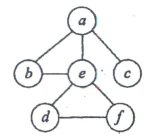
\includegraphics[width=0.3\textwidth]{../../figure/exercisePicPDF/chapter7/7-53.pdf}
            \caption{深度优先遍历}
            \label{fig:7-53}
    \end{figure}

        A. 5 个 \quad B. 4 个 \quad C. 3 个 \quad D. 2 个  
    
        答案:\textcolor{red}{B}

        解析:\\
        深度优先遍历(DFS)是一种递归或使用栈的遍历方式,遵循“尽可能深地搜索每个分支”的原则。\\
        根据图\ref{fig:7-53}的结构,分析给出的 5 个序列是否符合以下规则:\\
        - 每个顶点在访问时,其相邻的未访问顶点优先被访问;\\
        - 访问顺序应符合深度优先的规则。\\
        经过逐一验证,符合深度优先遍历规则的序列共有 4 个。\\
        因此,答案为 B。
        \item 图\ref{fig:7-54}给出由 7 个顶点组成的无向图。从顶点 1 出发,对它进行深度优先遍历得到的序列是( );而进行广度优先遍历得到的顶点序列是( )。  
        【中科院软件所 1999 六、2(2 分)】  

        \begin{figure}[h!]
            \centering
            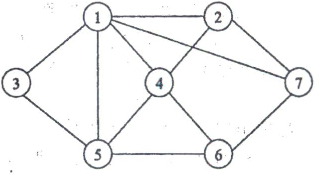
\includegraphics[width=0.3\textwidth]{../../figure/exercisePicPDF/chapter7/7-54.pdf}
            \caption{深度优先遍历}
            \label{fig:7-54}
    \end{figure}
        A. 深度优先:$1, 3, 5, 4, 2, 6, 7$;广度优先:$1, 5, 3, 4, 2, 6, 7$  

        B. 深度优先:$1, 3, 4, 7, 6, 5, 2$;广度优先:$1, 7, 2, 6, 4, 5, 3$  

        C. 深度优先:$1, 5, 3, 4, 2, 7, 6$;广度优先:$1, 3, 5, 4, 2, 7, 6$  

        D. 以上答案均不正确  
    
        答案:\textcolor{red}{A}

        解析:\\
        深度优先遍历(DFS)是一种递归或使用栈的遍历方式,遵循“尽可能深地搜索每个分支”的原则。\\
        广度优先遍历(BFS)是一种按层次逐层访问图中顶点的遍历方式,通常使用队列作为辅助数据结构。\\
        根据图\ref{fig:7-54}的结构,分析如下:\\
        - 深度优先遍历从顶点 1 出发,依次访问 $1 \to 3 \to 5 \to 4 \to 2 \to 6 \to 7$;\\
        - 广度优先遍历从顶点 1 出发,依次访问 $1 \to 5 \to 3 \to 4 \to 2 \to 6 \to 7$。\\
        因此,答案为 A。
        \item 下面哪一方法可以判断出一个有向图是否有环(回路)?  
    【东北大学 2000 四、2(4 分)】

    A. 深度优先遍历  
    B. 拓扑排序  
    C. 求最短路径  
    D. 求关键路径

    答案:\textcolor{red}{B}

    解析:\\
    拓扑排序只能对无环有向图成功,若尝试对有环图进行拓扑排序时会发现仍有入度不为 0 的顶点无法入队,由此可判断存在回路;\\
    虽然深度优先遍历也可通过检测“回边”判断环,但本题选项更明确对应拓扑排序。\\

\item 判断有向图是否有回路,除了可以用拓扑排序外,还可以用( )。  
    【南京理工大学 2004 一、7(2 分)】

    A. 求关键路径的算法  
    B. 广度优先遍历算法  
    C. 求最短路径的算法  
    D. 深度优先遍历算法

    答案:\textcolor{red}{D}

    解析:\\
    在 DFS 中,若在当前递归栈中再次遇到已标记为“正在访问”的顶点,则检测到回边,由此判断存在环;\\
    关键路径和最短路径算法并不专门用于环的检测,BFS 也无法直接检测回路。\\

\item 用邻接表表示图进行深度优先遍历时,通常是采用(  )来实现算法的。  
    【新疆大学 2017 二、8(2 分)】

    A. 栈  
    B. 队列  
    C. 树  
    D. 图

    答案:\textcolor{red}{A}

    解析:\\
    DFS 本质是“后进先出”的递归过程,可用显式栈模拟递归调用,依次保存待回溯的顶点;\\
    队列用于 BFS,树和图都不是辅助存储结构。\\

\item 在求边稠密的图的最小代价生成树时,采用(  )算法较合适。  
    【上海交通大学 2005 四、7(2 分)】

    A. 普里姆(Prim)  
    B. 克鲁斯卡尔(Kruskal)  
    C. 迪杰斯特拉(Dijkstra)  
    D. 其他

    答案:\textcolor{red}{A}

    解析:\\
    对于边数 $e$ 接近 $n^2$ 的稠密图,Prim 算法(用邻接矩阵和简单线性选最小边)时间 $O(n^2)$ 最优;\\
    Kruskal 需对所有边排序,耗时 $O(e\log e)\approx O(n^2\log n)$,不及 Prim 高效。\\

\item 在具有 $n$ 个顶点的图 $G$ 中,若最小生成树不唯一,则( )。  
    【电子科技大学 2008 一、2(2 分)】

    A. $G$ 的边数一定大于 $n-1$  
    B. $G$ 的权值最小的边一定有多条  
    C. $G$ 的最小生成树的代价不一定相等  
    D. 以上选项都不对

    答案:\textcolor{red}{D}

    解析:\\
    最小生成树不唯一的原因是存在不同权值相同的边可互换,但边数可等于 $n-1$ 也可大于 $n-1$;\\
    权值最小的边不必多条,且所有最小生成树的总代价必相等;故 A、B、C 均不成立。\\

\item 关于 Dijkstra 和 Floyd 算法的叙述中,不正确的是( )。  
    【南京理工大学 2000 一、21(1.5 分)】

    1. 求从指定源点到其余各顶点的 Dijkstra 最短路径算法中弧上权不能为负的原因是在实际应用中无意义  
    2. 利用 Dijkstra 求每一对不同顶点之间的最短路径的算法时间复杂度是 $O(n^2)$(图用邻接矩阵表示)  
    3. Floyd 求每对不同顶点对的算法中允许弧上的权为负,但不能有权和为负的回路

    A. 1  
    B. 2  
    C. 3  
    D. 以上都不正确

    答案:\textcolor{red}{B}

    解析:\\
    1 项虽表述不严,但可认为 Dijkstra 对负权限制主要源于算法正确性要求,而非“应用无意义”,可视为正确;\\
    2 项错误——单次 Dijkstra 为 $O(n^2)$,若对所有源点重复执行则为 $O(n^3)$;\\
    3 项正确——Floyd 允许负权边但须无负权回路以保证最短路径定义成立。\\

\item 当各边上的权值(  )时,Dijkstra 算法可以用来求解最短路径问题。  
    【中科院计算所 2000】

    A. 均相等  
    B. 均互不相等  
    C. 不一定相等

    答案:\textcolor{red}{C}

    解析:\\
    Dijkstra 算法只要求所有边权非负,无需相等或互不相等,因此权值可以任意非负分布;\\
    故选“不一定相等”。\\

\item 求解最短路径的 Floyd 算法的时间复杂度为( )。  
    【合肥工业大学 1999 二、2(2 分);中南大学 2005 一、8(2 分)】

    A. $O(n)$  
    B. $O(n+e)$  
    C. $O(n^2)$  
    D. $O(n^3)$

    答案:\textcolor{red}{D}

    解析:\\
    Floyd 算法三重嵌套循环遍历 $k,i,j$,故时间复杂度 $O(n^3)$。\\

\item 已知有向图 $G=(V,E)$,其中  
$V=\{V_1,\dots,V_7\}$,  
$E=\{(V_1,V_2),(V_1,V_3),(V_1,V_4),(V_2,V_5),(V_3,V_5),(V_3,V_6),(V_4,V_6),(V_5,V_7),(V_6,V_7)\}$。  
$G$ 的拓扑序列是( )。  
    【北京航空航天大学 2000 一、7(2 分)】

    A. $V_1,\;V_3,\;V_4,\;V_6,\;V_2,\;V_5,\;V_7$  
    B. $V_1,\;V_3,\;V_2,\;V_6,\;V_4,\;V_5,\;V_7$  
    C. $V_1,\;V_3,\;V_4,\;V_5,\;V_2,\;V_6,\;V_7$  
    D. $V_1,\;V_2,\;V_5,\;V_3,\;V_4,\;V_6,\;V_7$

    答案:\textcolor{red}{A}

    解析:\\
    初始仅 $V_1$ 入度为 0,先选 $V_1$;随后 $V_2,V_3,V_4$ 入度变 0,可任意先后,这里选 $V_3,V_4$;\\
    $V_6$ 仅依赖于 $V_3,V_4$,故下一;之后可选 $V_2$,再是 $V_5$,最后 $V_7$;故序列 A 合法。\\

\item 若一个有向图的邻接矩阵中主对角线以下的元素均为零,则该图的拓扑有序序列( )。  
    【中科院计算所 1998 二、6(2 分);中国科技大学 1998 二、6(2 分)】

    A. 存在  
    B. 不存在

    答案:\textcolor{red}{A}

    解析:\\
    矩阵主对角线以下为零意味着所有边均从编号小的顶点指向编号大的顶点,必为无环有向图,故一定存在拓扑序列。\\


    \item 在有向图 $G$ 的拓扑序列中,若顶点 $u$ 在顶点 $v$ 之前,则下列情形不可能出现的是( )。  
    【江苏大学 2006 一、1(2 分)】  

    A. $G$ 中存在弧 $(u, v)$  

    B. $G$ 中不存在弧 $(u, v)$  

    C. $G$ 中存在一条从 $u$ 到 $v$ 的路径  

    D. $G$ 中存在一条从 $v$ 到 $u$ 的路径  

    答案:\textcolor{red}{D}

    解析:\\
    拓扑排序是针对有向无环图(DAG)的一种线性排序,使得对于每一条有向边 $(u, v)$,顶点 $u$ 在排序中出现在顶点 $v$ 之前。\\
    - A. $G$ 中存在弧 $(u, v)$:符合拓扑排序规则,$u$ 是 $v$ 的前驱。\\
    - B. $G$ 中不存在弧 $(u, v)$:两者无直接依赖关系,顺序仍可能满足拓扑排序。\\
    - C. $G$ 中存在一条从 $u$ 到 $v$ 的路径:路径中 $u$ 必在 $v$ 之前,符合规则。\\
    - D. $G$ 中存在一条从 $v$ 到 $u$ 的路径:若存在此路径,则图中存在环,无法进行拓扑排序。\\
    因此,答案为 D。

\item 用邻接表表示图时,拓扑排序算法时间复杂度为( )。  
    【合肥工业大学 2000 一、2(2 分);南京理工大学 2001 一、9(1.5 分);青岛大学 2002 二、3(2 分)】 

    A. $O(n)$ \quad B. $O(n+e)$ \quad C. $O(n*e)$ \quad D. $O(n^2)$  

    答案:\textcolor{red}{B}

    解析:\\
    拓扑排序的时间复杂度取决于图的存储结构和遍历方式:\\
    - 邻接表存储时,初始化入度表的时间复杂度为 $O(n)$;\\
    - 遍历所有边以更新入度表的时间复杂度为 $O(e)$;\\
    - 每个顶点仅入队和出队一次,总时间复杂度为 $O(n)$。\\
    因此,总时间复杂度为 $O(n + e)$。

\item 在下列网中,( )是边不带权值的图。  
    【华南理工大学 2007】  

    A. 邮电图 \quad B. AOV 网 \quad C. 公路网 \quad D. AOE 网  

    答案:\textcolor{red}{B}

    解析:\\
    - AOV 网(Activity on Vertex Network)是以顶点表示活动的图,边表示活动间的优先关系,边不带权值。\\
    - AOE 网(Activity on Edge Network)是以边表示活动的图,边通常带权值表示活动的持续时间。\\
    - 邮电图和公路网通常是带权图,权值表示距离或费用。\\
    因此,答案为 B。

\item 关键路径是 AOE 网中( )。  
    【中南大学 2003 一、10(1 分)】  

    A. 从始点到终点的最短路径  

    B. 从始点到终点的最长路径  

    C. 从始点到终点的边数最多的路径  

    D. 从始点到终点的边数最少的路径  

    答案:\textcolor{red}{B}

    解析:\\
    关键路径是从始点到终点的最长路径,表示完成整个工程所需的最短时间。\\
    - A. 最短路径:错误,关键路径是最长路径。\\
    - B. 最长路径:正确,关键路径表示完成工程的最短时间。\\
    - C. 边数最多的路径:错误,关键路径与边数无关。\\
    - D. 边数最少的路径:错误,关键路径与边数无关。\\
    因此,答案为 B。

\item 下面关于求关键路径的说法不正确的是( )。  
    【南京理工大学 1998 一、12(2 分)】  

    A. 求关键路径是以拓扑排序为基础的  

    B. 一个事件的最早开始时间等于以该事件为尾的活动的最迟开始时间  

    C. 一个活动的总时差等于该活动的最迟开始时间减去最早开始时间  

    D. 关键活动一定位于关键路径上  

    答案:\textcolor{red}{B}

    解析:\\
    - A. 求关键路径是以拓扑排序为基础的:正确,关键路径算法需要对 AOE 网进行拓扑排序。\\
    - B. 一个事件的最早开始时间等于以该事件为尾的活动的最迟开始时间:错误,最早开始时间和最迟开始时间是独立计算的。\\
    - C. 一个活动的总时差等于该活动的最迟开始时间减去最早开始时间:正确,总时差的定义。\\
    - D. 关键活动一定位于关键路径上:正确,关键活动的总时差为 0,必在关键路径上。\\
    因此,答案为 B。

\item 下列关于 AOE 网的叙述中,不正确的是( )。  
    【北京大学 2016 一、8(2 分);北京工业大学 1999 一、1(2 分);哈尔滨工业大学 2004 二、3(1 分)】  

    A. 关键活动不按期完成就会影响整个工程的完成时间  

    B. 任何一个关键活动提前完成,那么整个工程将会提前完成  

    C. 所有的关键活动提前完成,那么整个工程将会提前完成  

    D. 某些关键活动若提前完成,那么整个工程将会提前完成  

    答案:\textcolor{red}{D}

    解析:\\
    - A. 关键活动不按期完成就会影响整个工程的完成时间:正确,关键活动决定工程工期。\\
    - B. 任何一个关键活动提前完成,那么整个工程将会提前完成:正确,关键活动决定工期。\\
    - C. 所有的关键活动提前完成,那么整个工程将会提前完成:正确,所有关键活动提前完成会缩短工期。\\
    - D. 某些关键活动若提前完成,那么整个工程将会提前完成:错误,仅部分关键活动提前完成未必缩短工期。\\
    因此,答案为 D。

\item 下列有关图的说法错误的是( )。  
    【中南大学 2003 二、19(1 分)】  

    A. 在有向图中,出度为 0 的结点称为叶子  

    B. 用邻接矩阵表示图容易判断任意两个结点之间是否有边相连,并求得各结点的度  

    C. 按深度方向遍历图和按先根次序遍历树类似,得到的结果是唯一的  

    D. 若有向图 $G$ 中从结点 $u$ 到结点 $v$ 有一条路径,则在图 $G$ 的结点的线性序列中结点 $u$ 必在结点 $v$ 之前  

    答案:\textcolor{red}{C}

    解析:\\
    - A. 在有向图中,出度为 0 的结点称为叶子:正确,出度为 0 的结点没有后继。\\
    - B. 用邻接矩阵表示图容易判断任意两个结点之间是否有边相连,并求得各结点的度:正确,邻接矩阵支持快速查询。\\
    - C. 按深度方向遍历图和按先根次序遍历树类似,得到的结果是唯一的:错误,深度优先遍历的结果依赖于邻接点的访问顺序,不唯一。\\
    - D. 若有向图 $G$ 中从结点 $u$ 到结点 $v$ 有一条路径,则在图 $G$ 的结点的线性序列中结点 $u$ 必在结点 $v$ 之前:正确,拓扑排序满足此性质。\\
    因此,答案为 C。

\item 下面的叙述中,不正确的是( )。  
    【吉林大学 2017 一、4(2 分)】  

    A. 任何一个关键活动不按期完成,就会影响整个工程的完成时间  

    B. 任何一个关键活动提前完成,将使整个工程提前完成  

    C. 所有关键活动都提前完成,将使整个工程提前完成  

    D. 所有关键活动不按期完成,就会影响整个工程的完成时间  

    答案:\textcolor{red}{B}

    解析:\\
    - A. 任何一个关键活动不按期完成,就会影响整个工程的完成时间:正确,关键活动决定工期。\\
    - B. 任何一个关键活动提前完成,将使整个工程提前完成:错误,仅一个关键活动提前完成未必缩短工期。\\
    - C. 所有关键活动都提前完成,将使整个工程提前完成:正确,所有关键活动提前完成会缩短工期。\\
    - D. 所有关键活动不按期完成,就会影响整个工程的完成时间:正确,关键活动决定工期。\\
    因此,答案为 B。

\item 采用邻接表存储的图的深度优先遍历算法类似二叉树的( )算法。  
    【北京大学 2015 一、6(1.5 分)】  

    A. 前序遍历 \quad B. 中序遍历 \quad C. 后序遍历 \quad D. 按层次遍历  

    答案:\textcolor{red}{A}

    解析:\\
    深度优先遍历(DFS)首先访问当前顶点,再递归访问其邻接顶点,类似于二叉树的前序遍历。\\
    因此,答案为 A。

\item 在一个无向图中,所有顶点的度之和等于边之和的( )倍。  
    【北京大学 2016 一、7(2 分)】  

    A. $\frac{1}{2}$ \quad B. 1 \quad C. 2 \quad D. 4  

    答案:\textcolor{red}{C}

    解析:\\
    在无向图中,每条边连接两个顶点,因此所有顶点的度之和等于边数的两倍。\\
    因此,答案为 C。

\item 在一个有向图中,所有顶点的度数之和与图的边数的比是( )。  
    【烟台大学 2019 一、15(2 分)】  

    A. 1:2 \quad B. 1:1 \quad C. 2:1 \quad D. 4:1  

    答案:\textcolor{red}{B}

    解析:\\
    在有向图中,每条边有一个起点和一个终点,因此所有顶点的出度和入度之和等于边数的两倍。\\
    因此,答案为 B。

\item 在一个包含 $n$ 个顶点的有向图中,如果所有顶点的出度之和为 $s$,则所有顶点的入度之和为( )。  
    【北京工业大学 2017 一、8(2 分)】  

    A. $n$ \quad B. $s$ \quad C. $2n$ \quad D. $s-1$  

    答案:\textcolor{red}{B}

    解析:\\
    在有向图中,每条边的起点贡献一个出度,终点贡献一个入度,因此所有顶点的出度之和等于入度之和。\\
    因此,答案为 B。

\item 若 $G$ 是一个具有 36 条边的非连通无向图(不含回路和多重边),则图 $G$ 的结点数至少是( )。  
    【北京大学 2015 一、7(1.5 分)】 

    A. 8 \quad B. 11 \quad C. 10 \quad D. 9  

    答案:\textcolor{red}{B}

    解析:\\
    对于非连通无向图,边数最多的情况下,图可以分为多个完全子图。\\
    - 若图中有 $n$ 个顶点,则最多可以分为 $\binom{n}{2}$ 条边。\\
    - 解不等式 $\binom{n}{2} \geq 36$,得 $n \geq 9$。\\
    因此,答案为 B。
\end{enumerate}

\end{document}
